\pgfplotsset{compat=newest}
\pgfplotsset{
  layers/my layer set/.define layer set={
    background,
    main,
    foreground
  }{},
  set layers=my layer set,
}

\begin{center}
  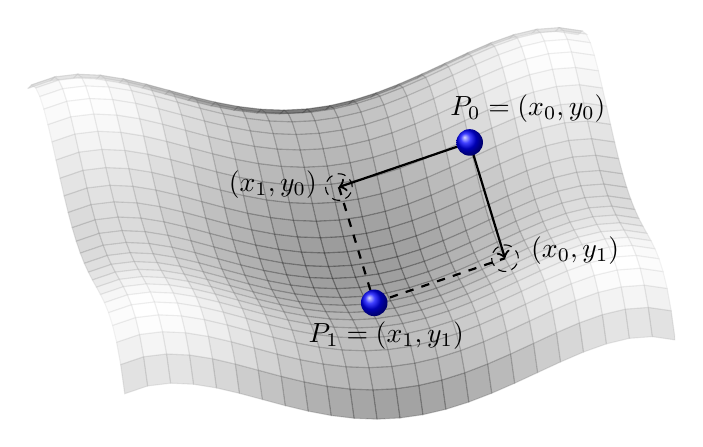
\begin{tikzpicture}[
      scale = 1.2
    ]
    \begin{axis}[
        view={-10}{60},
        zmin=-2,
        zmax=5,
        colormap/blackwhite,
        hide axis,
        xlabel=$x$,
        ylabel=$y$,
        z buffer=sort
      ]


      \addplot3 [
          surf,
          shader=faceted,
          opacity=0.2,
          fill opacity=0.4,
          samples=25,
          domain=-2:2,
          y domain=-2:2,
        ] {1.5*x^2 + 1.2*y^2 - 0.25*x^4 - 0.3*y^4};
      
      \addplot3 [
        draw=none, 
        mark=ball, 
        mark size=4, 
        z
      ] table[row sep=crcr] {%
          1     0.8     1.895\\
          0.05  -0.655  0.463 \\
        };
      
      \addplot3 [
        draw = none, 
        mark = o, 
        mark size=4,
        mark options = {
          densely dashed
        },
        z
      ] table[row sep=crcr] {%
          0.05  0.8   0.649 \\
          1     -0.655   1.710 \\
        };
      
      \addplot3 [
        <-, 
        thick, 
        black,
        z
      ] coordinates {
        (1,0.8,1.895) 
        (0.05,0.8, 0.649)
      };
      
      \addplot3 [
        -, 
        thick, 
        black,
        dashed,
        z
      ] coordinates {
        (0.05,0.8, 0.649)
        (0.05,-0.655, 0.463)
      };
      
      \addplot3 [
        ->, 
        thick, 
        black,
        z
      ] coordinates {
        (1,0.8,1.895) 
        (1,-0.655, 1.710)
      };
      
      \addplot3 [
        -, 
        thick, 
        black,
        dashed,
        z
      ] coordinates {
        (1,-0.655, 1.710)
        (0.05,-0.655, 0.463)
      };

      % \node[font=\bfseries, above] at (axis cs: 1.2, 0.8, 1.895) {$P_0 = (x_0, y_0)$};
      % \node[font=\bfseries, below] at (axis cs: 0.05, -0.655, 0.463) {$P_1 = (x_1, y_1)$};
    \end{axis}

    % \draw[step=1cm,gray,very thin] (0,0) grid (12,8);
    
    \node[font=\bfseries] at (5.5,4.1) {$P_0 = (x_0, y_0)$};
    \node[font=\bfseries] at (4,1.7) {$P_1 = (x_1, y_1)$};
    
    \node[font=\bfseries] at (6,2.6) {$(x_0, y_1)$};
    \node[font=\bfseries] at (2.8,3.3) {$(x_1, y_0)$};

  \end{tikzpicture}
\end{center}

